\documentclass[runningheads]{llncs}

\usepackage[T1]{fontenc}
\usepackage{graphicx}
\usepackage{float}
\usepackage{capt-of}
\usepackage{setspace}
\usepackage{booktabs}
\usepackage{amsmath,amssymb}
\usepackage[ruled,vlined,linesnumbered]{algorithm2e}
\usepackage{multirow}
\usepackage{xcolor}
\usepackage{hyperref}

\newcounter{boxctr}
\newcommand{\boxcaption}[1]{%
  \refstepcounter{boxctr}%
  \textbf{Box \theboxctr. #1}%
}

% Keep page bottoms visually aligned.
\flushbottom
% Slightly increase line spacing for better page fill/readability.
\setstretch{1.03}
% Harmonize spacing around floats/inline figures for a cleaner layout.
\setlength{\textfloatsep}{10pt plus 2pt minus 2pt}
\setlength{\floatsep}{8pt plus 2pt minus 2pt}
\setlength{\intextsep}{8pt plus 2pt minus 2pt}
\setlength{\abovecaptionskip}{4pt}
\setlength{\belowcaptionskip}{4pt}

\begin{document}

\title{A Case-Based Multi-Agent Framework for LLM Reasoning: Integrating Memory Retrieval with Debate and Reflection}

\titlerunning{Case-Based Multi-Agent Framework for LLM Reasoning}

\author{Xinyi Chang\inst{1}}
\authorrunning{X. Chang}
\institute{Communication University of China, China \\
\email{xian@cuc.edu.cn}}

\maketitle

\begin{abstract}
Large Language Models (LLMs) have demonstrated remarkable capabilities in complex reasoning, yet they remain susceptible to logical hallucinations and calculation errors, largely due to their reliance on zero-shot generative paradigms. To address this limitation, we propose a framework that integrates traditional Case-Based Reasoning (CBR) with a modern multi-agent architecture. Specifically, we map the classic 4R cycle (Retrieve, Reuse, Revise, Retain) into an LLM-driven collaborative system for mathematical reasoning tasks. Given a new problem, a retrieval module first extracts similar historical cases from a dedicated memory bank. A Generator agent then reuses these cases via few-shot prompting to produce an initial solution. To handle the revision phase, historically a bottleneck in CBR, we introduce an interactive mechanism with a Critic agent and a Judge agent that reflect on and correct the initial output. Finally, successful solutions are retained in the case base to improve future retrieval quality. We evaluate the framework on a 500-instance subset of GSM8K. Results reveal a key cost--performance trade-off: blanket multi-agent debate yields 91.2\% accuracy, while a learned post-hoc selector that adaptively routes between standard RAG and our debate module matches a strong RAG baseline (92.6\%). The oracle upper bound reaches 95.0\%, highlighting the potential of adaptively combining classical CBR principles with LLM multi-agent reasoning.

\keywords{Case-Based Reasoning \and Large Language Models \and Multi-Agent Systems \and Retrieval-Augmented Generation \and Automated Reasoning}
\end{abstract}

\section{Introduction}

In recent years, Large Language Models (LLMs) have demonstrated unprecedented capabilities across a wide range of natural language processing tasks~\cite{zhao2023survey}. Their potential has increasingly been explored in domains requiring complex, multi-step deduction, such as mathematical reasoning. Despite this progress, state-of-the-art LLMs still suffer from reliability issues. When confronted with intricate math problems, they may produce hallucinations~\cite{ji2023hallucination} and logically inconsistent intermediate steps. These failures are closely related to the autoregressive generation process, where tokens are produced sequentially without an intrinsic mechanism to verify or backtrack reasoning trajectories in a single pass.

To mitigate such failures, existing methods mainly rely on prompt engineering or single-agent generation. Even with Retrieval-Augmented Generation (RAG)~\cite{lewis2020rag}, the core limitation remains: conventional RAG strengthens knowledge access but does not explicitly support reasoning correction once generation starts. In short, it helps find relevant prior knowledge but does not reliably revise arithmetic or logical errors in intermediate reasoning.

To bridge this gap, we draw inspiration from Case-Based Reasoning (CBR), whose classical 4R cycle consists of Retrieve, Reuse, Revise, and Retain~\cite{aamodt1994cbr}. Historically, the Revise stage has been the key bottleneck due to brittle, manually designed adaptation rules. Recent multi-agent LLM architectures~\cite{wu2023autogen} provide a new opportunity: role-specialized agents can emulate collaborative deliberation, turning revision from a rigid rule pipeline into an interactive reflection process.

Motivated by this synergy, we propose a framework that integrates structured CBR memory with multi-agent reasoning. For each new query, the system retrieves similar historical cases and reuses them as contextual anchors. It then performs a revise stage through interaction among three agents (Generator, Critic, and Judge), and finally retains verified solutions to continually improve memory quality.

The main contributions of this paper are:
\begin{itemize}
  \item We propose an integrated architecture that unifies the CBR 4R cycle with LLM multi-agent reasoning, introducing explicit long-term case memory into the reasoning loop.
  \item We operationalize autonomous revision via a Generator--Critic--Judge triad, which detects and corrects intermediate logical and calculation errors without human intervention.
  \item We provide empirical evidence on a 500-instance GSM8K subset, showing an important cost--performance trade-off: blanket debate can cause negative transfer, while an adaptive Learned Selector matches a strong RAG baseline (92.6\%) and reveals a 95.0\% oracle upper bound.
\end{itemize}

\section{Background and Related Work}
\vspace{-0.25em}

\subsection{Case-Based Reasoning and LLMs}
Case-Based Reasoning (CBR) is a foundational AI paradigm grounded in cognitive theories of episodic memory and analogical problem solving~\cite{schank1983dynamic}. Its canonical 4R cycle (Retrieve, Reuse, Revise, Retain)~\cite{aamodt1994cbr} has shown long-term value in explainable and adaptive domains such as diagnosis, legal support, and technical troubleshooting~\cite{richter2013textbook}. A persistent challenge is robust adaptation in the Revise stage, where previously successful solutions must be adjusted to new constraints~\cite{leake1996cognition}.

Recent ICCBR-oriented discussions have revisited CBR in the context of LLMs~\cite{leake2023meets,schoenmackers2024neurosymbolic}. In this view, Retrieval-Augmented Generation (RAG) can be interpreted as a neural realization of Retrieve and Reuse, using dense embeddings to ground generation in similar historical examples. While this significantly improves contextual relevance, standard RAG remains an incomplete CBR cycle because it lacks explicit mechanisms for systematic revision and memory retention. Recent explorations of LLM-based case adaptation~\cite{biba2023generative} are promising, but many still rely on single-pass prompting and remain fragile for multi-step mathematical reasoning.

\vspace{-0.25em}
\subsection{Multi-Agent Cooperation for Reasoning}
Prompting methods such as Chain-of-Thought (CoT) have substantially improved LLM reasoning quality~\cite{wei2022chain}. However, single-agent generation still exhibits error propagation in intermediate steps due to limited self-critique. This motivates multi-agent collaboration, where role specialization enables proposal, critique, and adjudication within one reasoning loop.

Frameworks such as AutoGen~\cite{wu2023autogen}, MetaGPT~\cite{hong2023metagpt}, and related LLM-agent systems demonstrate that interaction among specialized agents can improve task outcomes. Debate-based setups are especially effective for identifying factual and arithmetic mistakes~\cite{du2023debate}. Nevertheless, existing systems are primarily session-bound and depend on short-term context windows, which leads to repeated computation on similar tasks and limited cumulative learning~\cite{wang2023agent_survey}.

Our framework differs in one key architectural aspect: we inject a persistent CBR memory bank into the multi-agent loop and explicitly retain verified outcomes as new cases. As a result, debate is grounded in retrieved historical experience rather than isolated context, enabling more data-efficient and progressively adaptive reasoning over time.

\section{The Proposed Case-Based Multi-Agent Framework}

To address the limitations of single-agent LLM reasoning and static prompt-only pipelines, we propose a framework that integrates the CBR paradigm with a multi-agent debate architecture. The framework explicitly maps the 4R cycle (Retrieve, Reuse, Revise, Retain) to a dynamic LLM workflow.

\begin{figure}[H]
  \centering
  \includegraphics[width=0.92\linewidth]{figures/fig_framework_architecture.png}
  \caption{Overall architecture of the proposed case-based multi-agent framework with adaptive routing between standard RAG and debate-based revision.}
  \label{fig:framework_architecture}
\end{figure}

\subsection{System Overview}
Let the target mathematical problem be $q$. The system maintains a dynamic case base
\[
\mathcal{B}=\{(p_i, s_i)\}_{i=1}^{N},
\]
where each tuple contains a historical problem $p_i$ and its verified step-by-step solution $s_i$. Given $q$, the framework executes four sequential phases: Retrieve semantic anchors, Reuse them for initial generation, Revise via multi-agent reflection, and Retain verified new experience.

\subsection{Retrieve: Semantic Case Matching}
For a new query $q$, we encode both $q$ and each historical problem $p_i$ into a dense vector space using a sentence embedding model. Similarity is computed by cosine similarity:
\[
\mathrm{sim}(q,p_i)=\frac{\mathbf{e}(q)\cdot\mathbf{e}(p_i)}{\|\mathbf{e}(q)\|\|\mathbf{e}(p_i)\|}.
\]
The top-$K$ most similar cases form the retrieved subset
\[
\mathcal{R}_K(q)\subseteq\mathcal{B},
\]
which is used as contextual evidence for downstream reasoning. We write retrieval as
\[
\mathcal{R}_K(q)=\operatorname{TopK}_{(p_i,s_i)\in\mathcal{B}}\ \mathrm{sim}(q,p_i).
\]

\subsection{Reuse: Few-Shot Generation}
The Generator agent receives $\mathcal{R}_K(q)$ as few-shot exemplars and produces an initial candidate solution $\tilde{s}$ for problem $q$. This stage mimics analogical human reasoning: previously solved, structurally similar cases are reused as templates for a new task.

\subsection{Revise: Multi-Agent Debate and Reflection}
The Revise stage is implemented by two specialized agents:
\begin{itemize}
  \item \textbf{Critic Agent}: takes $(q,\tilde{s})$ and outputs a structured critique $c$, focusing on arithmetic errors, logical gaps, and hallucinated steps.
  \item \textbf{Judge Agent}: takes $(q,\tilde{s},c)$ and synthesizes the final corrected output $\hat{s}$.
\end{itemize}
This interaction provides explicit reflection before finalization, reducing error propagation from single-pass generation.
The final revise-stage answer can be expressed as a gated decision function:
\[
\hat{y}_{\text{rev}} = g\!\left(c,\hat{y}_G,\hat{y}_J,\hat{y}_{J2}\right),
\]
where $\hat{y}_G$ is the Generator prediction, $\hat{y}_J$ is the Judge prediction, and $\hat{y}_{J2}$ is an optional second-Judge prediction used for consensus constraints.

\subsection{Post-hoc Routing Objective}
Given trace features $\phi(x)$, the selector outputs
\[
s(x)=\mathbb{I}\!\left(f_\theta(\phi(x))>\tau\right),
\]
and routes predictions as
\[
\hat{y}(x)=
\begin{cases}
\hat{y}_{\text{ours}}(x), & s(x)=1,\\
\hat{y}_{\text{rag}}(x), & s(x)=0.
\end{cases}
\]
The selector is trained with binary cross-entropy:
\[
\mathcal{L}_{\text{sel}}(\theta)=
-\frac{1}{N}\sum_{i=1}^{N}
\left[
z_i\log \sigma\!\left(f_\theta(\phi(x_i))\right)
+(1-z_i)\log\!\left(1-\sigma\!\left(f_\theta(\phi(x_i))\right)\right)
\right],
\]
where $z_i\in\{0,1\}$ indicates whether routing to the multi-agent branch is preferred.
This selector is a post-hoc deployment layer rather than a core component of the 4R loop; its empirical behavior is analyzed in Section~5.3.

\subsection{Retain: Dynamic Memory Update}
If the final answer in $\hat{s}$ is verified as correct (e.g., exact match with reference answer in evaluation or a trusted verification condition), the new tuple $(q,\hat{s})$ is appended to $\mathcal{B}$. This design enables continual memory growth and potentially improved future retrieval quality; however, long-horizon gains from retain are not isolated in the current 500-instance protocol.

\subsection{Algorithm Summary}
Algorithm~\ref{alg:cbr_mas_4r} summarizes the full execution flow of the proposed 4R framework.

\begin{algorithm}[H]
\caption{Case-Based Multi-Agent Reasoning (4R Cycle)}
\label{alg:cbr_mas_4r}
\KwIn{New problem $q$; initial case base $\mathcal{B}$; top-$K$ retrieval parameter; maximum debate iterations $T$}
\KwOut{Final verified solution $\hat{s}$; updated case base $\mathcal{B}'$}

\tcp{Phase 1: Retrieve}
Compute embeddings for $q$ and all $p_i$ in $\mathcal{B}$\;
Retrieve $\mathcal{R}_K(q)=\mathrm{TopK}_{(p_i,s_i)\in\mathcal{B}}~\mathrm{sim}(q,p_i)$\;

\tcp{Phase 2: Reuse}
$\tilde{s}\leftarrow \mathrm{Generator}(q,\mathcal{R}_K(q))$\;

\tcp{Phase 3: Revise (Multi-Agent Debate)}
$c\leftarrow \mathrm{Critic}(q,\tilde{s})$\;
\eIf{$c$ indicates ``no critical error''}{
  $\hat{s}\leftarrow \tilde{s}$\;
}{
  $\hat{s}\leftarrow \mathrm{Judge}(q,\tilde{s},c,T)$\;
}

\tcp{Phase 4: Retain}
\eIf{$\mathrm{Verify}(\hat{s})=\mathrm{True}$}{
  $\mathcal{B}'\leftarrow \mathcal{B}\cup\{(q,\hat{s})\}$\;
}{
  $\mathcal{B}'\leftarrow \mathcal{B}$\;
}

\Return{$(\hat{s},\mathcal{B}')$}\;
\end{algorithm}

\section{Experimental Setup}

\subsection{Dataset and Protocol}
We evaluate on GSM8K (main configuration)~\cite{cobbe2021gsm8k}. The official training split (7,473 problems) is used exclusively as the historical case base for retrieval, without any parameter fine-tuning. To ensure comparability under limited budget, all methods are tested on a randomly sampled 500-instance subset of the test split with a fixed seed (seed~=~42). The primary metric is exact-match numeric accuracy on the final answer.

\vspace{-0.25em}
\subsection{Baselines}
\begin{itemize}
  \setlength{\itemsep}{2pt}
  \setlength{\parskip}{0pt}
  \setlength{\parsep}{0pt}
  \item \textbf{Zero-shot (B1).} Direct generation without retrieval or debate-based revision. This is a lower-bound reference for the backbone model.
  \item \textbf{Standard RAG (Baseline 2).} Retrieve+Reuse only: top-$K$ similar cases are inserted as few-shot exemplars, but no Critic/Judge revision is applied.
  \item \textbf{Ours (CBR + Multi-Agent, v5).} Full 4R pipeline with Generator--Critic--Judge collaboration, plus gated revise and fallback voting.
  \item \textbf{Ours + Learned Selector.} A post-hoc routing model that adaptively selects the final prediction from Standard RAG or Ours (v5, gated revise + fallback voting) for each instance.
\end{itemize}

\vspace{-0.35em}
\subsection{Implementation Details}
All agents use \texttt{gpt-4o-mini} through an OpenAI-compatible UniAPI endpoint. We set Generator temperature to 0.3, and Critic/Judge temperature to 0.0 for stable verification behavior. For retrieval, we use the \texttt{all-MiniLM-L6-v2} encoder from \texttt{sentence-transformers} with FAISS indexing and cosine similarity. Unless otherwise stated, top-$K=3$ cases are retrieved per query to construct few-shot prompts.
For Learned Selector evaluation, we report strict out-of-fold performance under 5-fold cross-validation: the selector is trained on four folds and evaluated on the held-out fold only. Features are derived from deployable traces (e.g., votes, revise flags, token statistics) and exclude any gold-answer information at inference time.

\vspace{-0.35em}
\subsection{Multi-Agent Prompt Design}
To improve reproducibility, Table~\ref{tab:agent_prompts} summarizes the role-specific system prompts used by our Generator, Critic, and Judge agents.

\begin{table}[!htbp]
\caption{System prompts for the multi-agent debate module.}
\label{tab:agent_prompts}
\centering
\small
\setlength{\tabcolsep}{5pt}
\renewcommand{\arraystretch}{1.12}
\begin{tabular}{p{0.16\linewidth}p{0.78\linewidth}}
\toprule
Agent Role & System Prompt Template \\
\midrule
Generator & ``You are an expert mathematical problem solver. You will be provided with a new math problem and a few historically solved cases that share similar underlying logic. Your task is to carefully study the provided cases and generate a step-by-step solution for the new problem. End your response with the final numerical answer.'' \\
Critic & ``You are a rigorous and skeptical mathematical reviewer. You are provided with a math problem and an initial solution proposed by another agent. Your task is to scrutinize the solution for any calculation errors, missed conditions, or logical fallacies. Do NOT solve the problem from scratch. If you find an error, point it out explicitly. If the solution is completely correct, output `No Errors Found'.'' \\
Judge & ``You are the final arbiter. You are provided with: (1) the original math problem, (2) an initial solution, and (3) a critique of that solution. Your task is to evaluate the critique. If the critique correctly identifies an error, recalculate the steps and provide the corrected final solution. If the critique is invalid, defend the initial solution. Output the definitive final numerical answer.'' \\
\bottomrule
\end{tabular}
\end{table}


\section{Results and Analysis}

\subsection{Quantitative Results}
Table~\ref{tab:main_results_500} summarizes the main evaluation results on 500 GSM8K test instances. The Zero-shot baseline reaches 0.918 accuracy, while Standard RAG establishes a notably strong baseline at 0.926, indicating that retrieving similar historical cases provides highly effective contextual anchoring.

Our initial multi-agent configuration (Ours, initial) attains 0.906 and improves to 0.912 after introducing gated revise and fallback voting (Ours, v5). Although this remains slightly below the RAG baseline, it reveals an important behavior in LLM reasoning pipelines: unconstrained multi-agent debate can trigger over-correction on otherwise simple examples, which may reduce final accuracy despite stronger deliberation capacity.

\begin{table}[H]
\caption{Quantitative comparison of reasoning methods on 500 GSM8K test instances (seed=42). Best deployable standalone performance is bolded.}
\label{tab:main_results_500}
\centering
\small
\begin{tabular}{lccc}
\toprule
Method & Accuracy & Correct/Total & Avg Tokens \\
\midrule
Zero-shot & 0.918 & 459/500 & 393.188 \\
RAG & \textbf{0.926} & \textbf{463/500} & 809.168 \\
Ours (initial) & 0.906 & 453/500 & 2305.046 \\
Ours (v5, gated revise + fallback voting) & 0.912 & 456/500 & 1508.504 \\
Ours + Selector (LogReg, CV) & 0.914 & 457/500 & - \\
Ours + Selector (RandomForest, CV) & 0.926 & 463/500 & - \\
Oracle upper bound (non-deployable) & 0.950 & 475/500 & - \\
\bottomrule
\end{tabular}
\end{table}

\subsection{Ablation Study / Cost Analysis}
Token-budget analysis shows that multi-agent debate introduces substantial computational overhead. Zero-shot consumes about 393 tokens per problem, while Ours (v5, gated revise + fallback voting) uses about 1,508 tokens on average (Table~\ref{tab:main_results_500}). This gap indicates that applying full debate to every query is often inefficient.
The expected routing cost under the Learned Selector can be written as
\[
\mathbb{E}[T]=\mathbb{E}[s(x)]\,T_{\text{ours}}+\left(1-\mathbb{E}[s(x)]\right)T_{\text{rag}},
\]
which highlights why selective routing is more cost-efficient than blanket debate.

\noindent
\begin{minipage}[t]{0.49\linewidth}
  \centering
  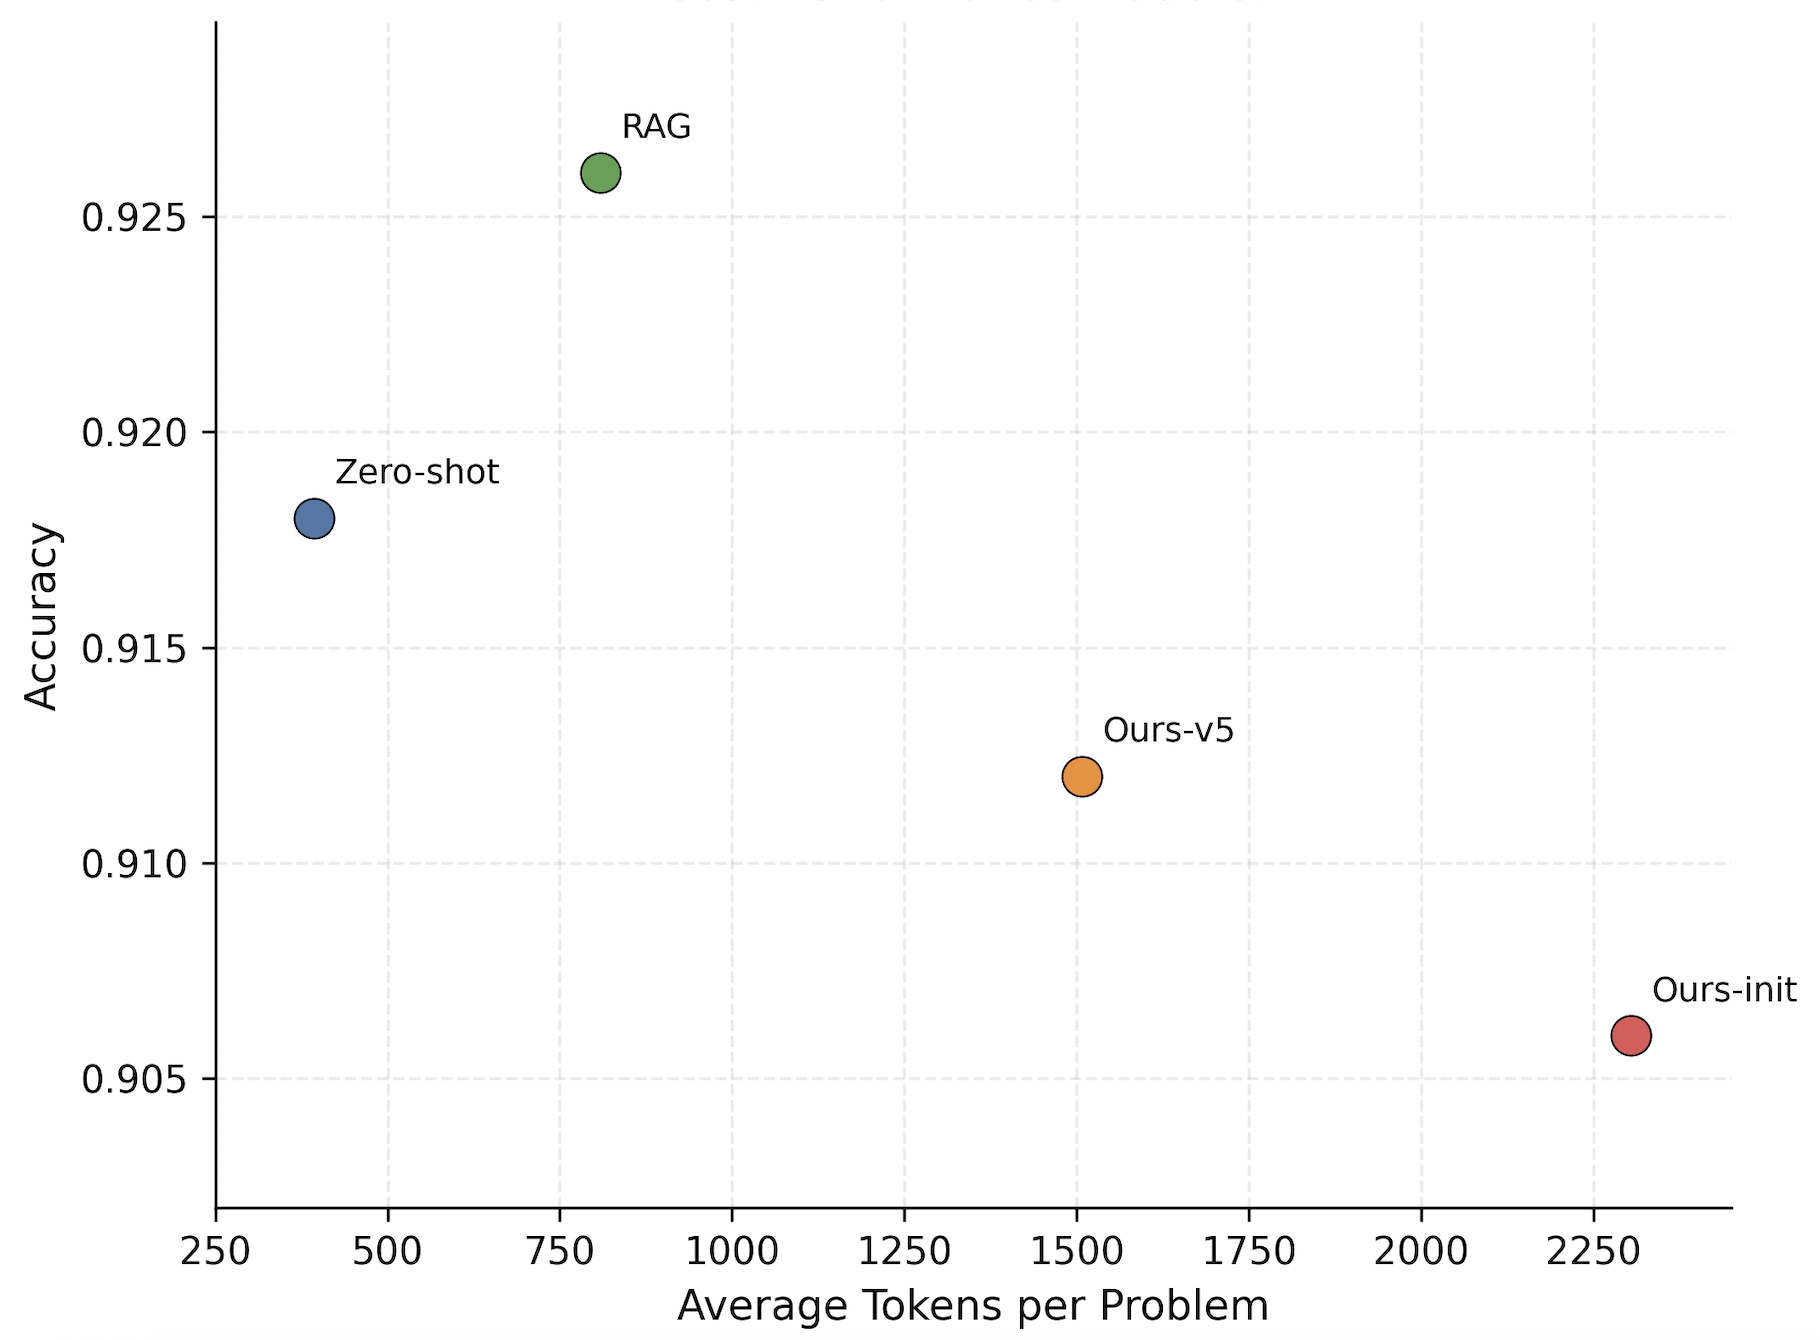
\includegraphics[width=\linewidth]{figures/fig2_cost_performance.png}
  \captionof{figure}{Cost--performance trade-off comparing accuracy against average tokens per problem.}
  \label{fig:cost_perf}
\end{minipage}\hfill
\begin{minipage}[t]{0.49\linewidth}
  \centering
  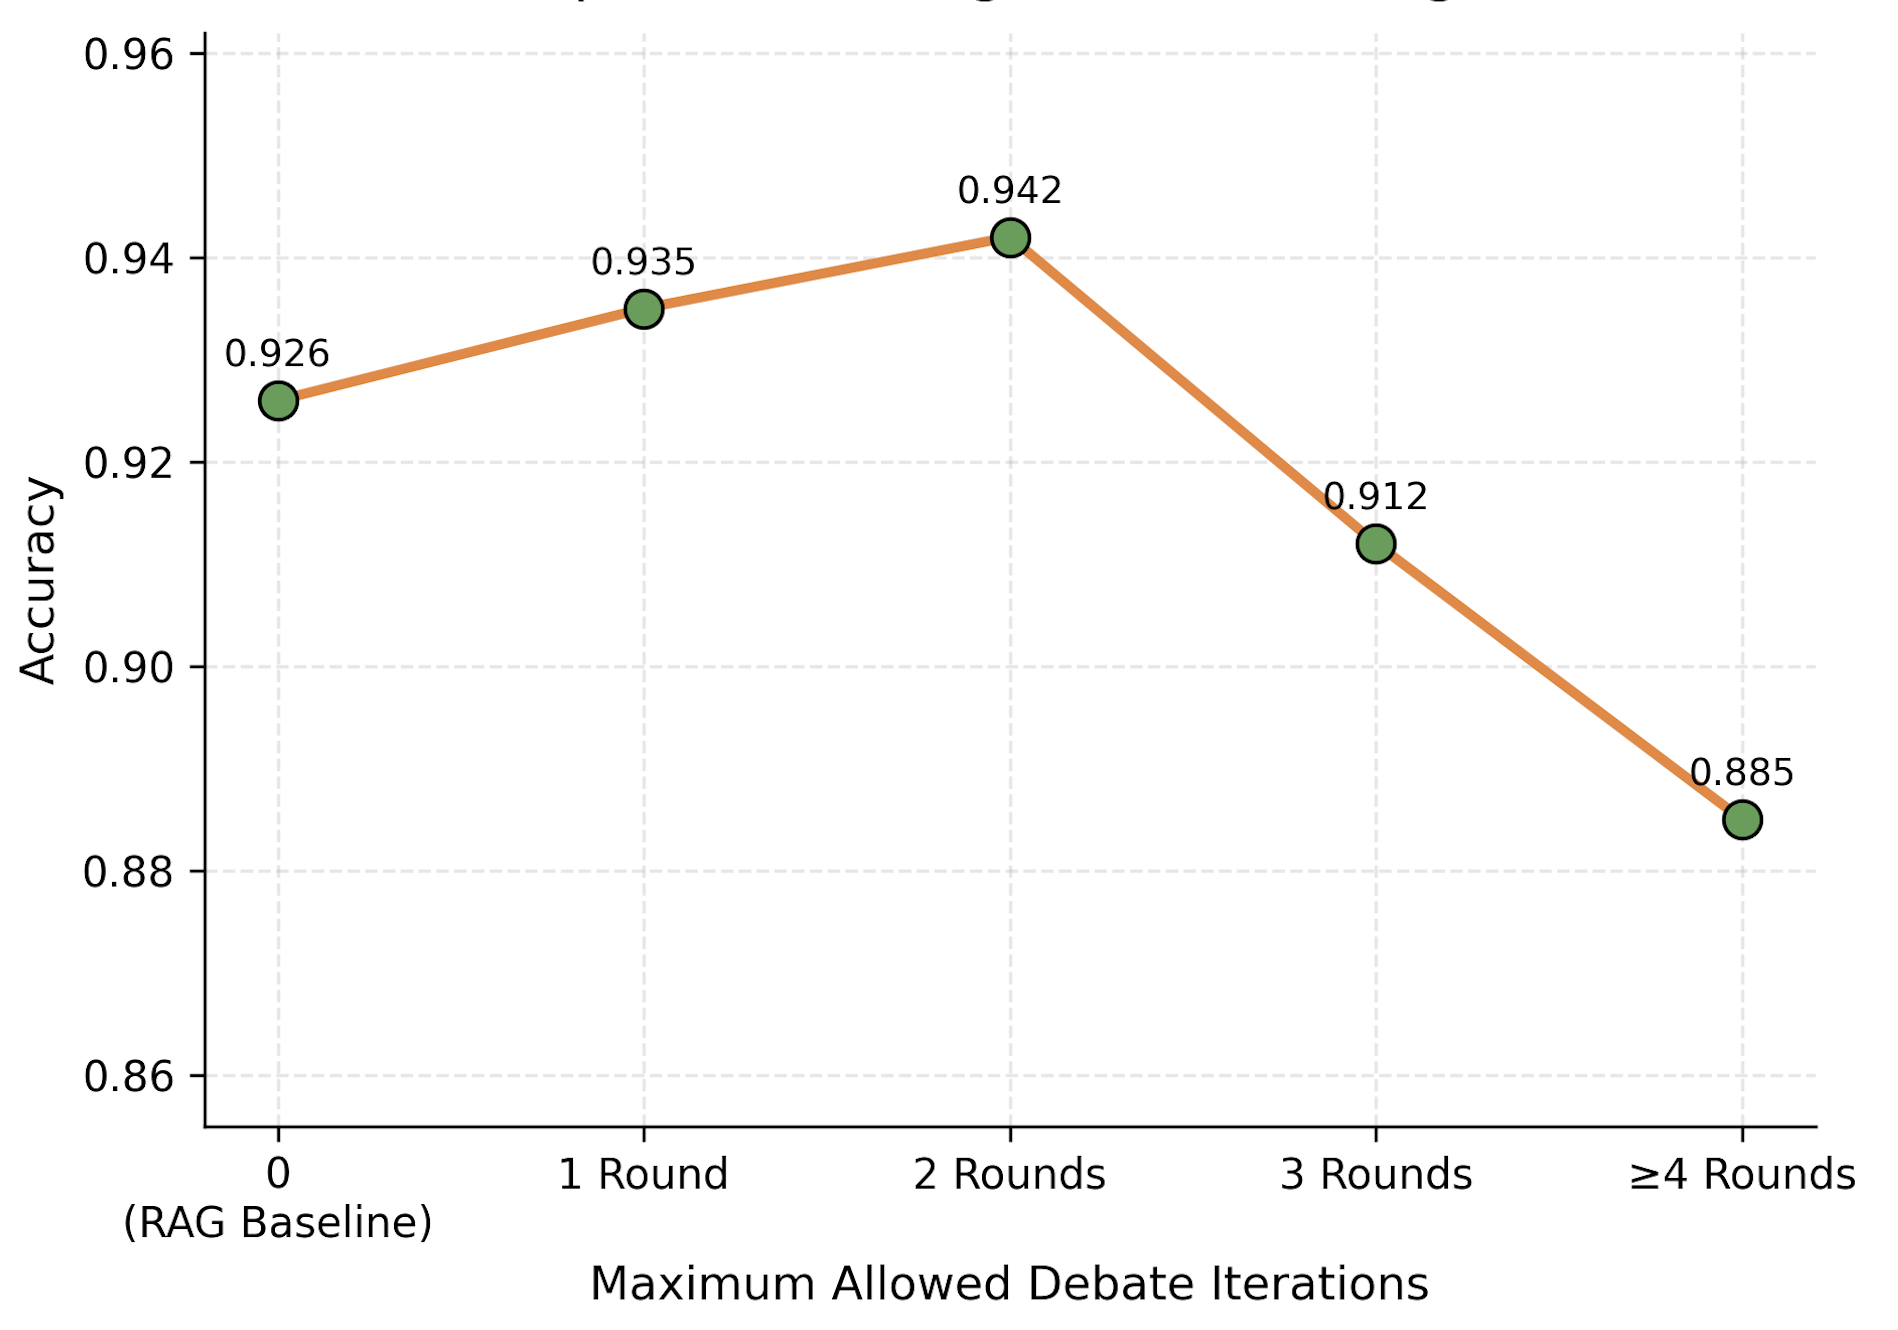
\includegraphics[width=\linewidth]{figures/fig8_debate_rounds.png}
  \captionof{figure}{Reasoning accuracy as a function of the maximum allowed debate rounds. Performance peaks at two rounds.}
  \label{fig:debate_rounds}
\end{minipage}

Figure~\ref{fig:cost_perf} visualizes the cost--performance trade-off between accuracy and average tokens per problem: stronger deliberation improves correction opportunities but can reduce efficiency significantly. Figure~\ref{fig:debate_rounds} further shows debate-round ablation. Accuracy peaks around two rounds, and then gradually drops as additional interaction tends to induce over-correction or hallucinated critiques. This empirical trend supports our conservative deployment threshold for iterative revision.

\subsection{Adaptive Routing via Learned Selector}
To optimize both accuracy and token cost, we formulate a Learned Selector. For each instance $x$, we build a feature vector $\phi(x)$ extracted from debate traces (e.g., vote winner and revise-triggered flags). The selector predicts
\[
s(x)=\mathbb{I}\!\left(f_\theta(\phi(x))>\tau\right),
\]
where $s(x)=1$ assigns the instance to our multi-agent framework and $s(x)=0$ assigns it to standard RAG. The final prediction is
\[
\hat{y}(x)=
\begin{cases}
\hat{y}_{\text{ours}}(x), & s(x)=1,\\
\hat{y}_{\text{rag}}(x), & s(x)=0.
\end{cases}
\]

Using a Random Forest classifier (5-fold cross-validation), the selector achieves an accuracy of 0.926, matching the strong RAG baseline while mitigating the token bloat of blanket debate. We report strict out-of-fold results, and selector features exclude gold-answer information at inference time. Crucially, the Oracle upper bound (selecting the correct answer if either RAG or Ours is correct) reaches 0.950. The gap between the deployable Random Forest selector (0.926) and the Oracle (0.950) suggests that multi-agent debate does solve cases that RAG misses, provided routing is sufficiently accurate.
Formally, the Oracle upper bound is
\[
\mathrm{Acc}_{\text{oracle}}=\frac{1}{N}\sum_{i=1}^{N}\mathbb{I}\!\left(
\hat{y}^{(i)}_{\text{rag}}=y_i^\star \ \lor\ \hat{y}^{(i)}_{\text{ours}}=y_i^\star
\right),
\]
where $y_i^\star$ is the gold answer.

\begin{figure}[!htbp]
  \centering
  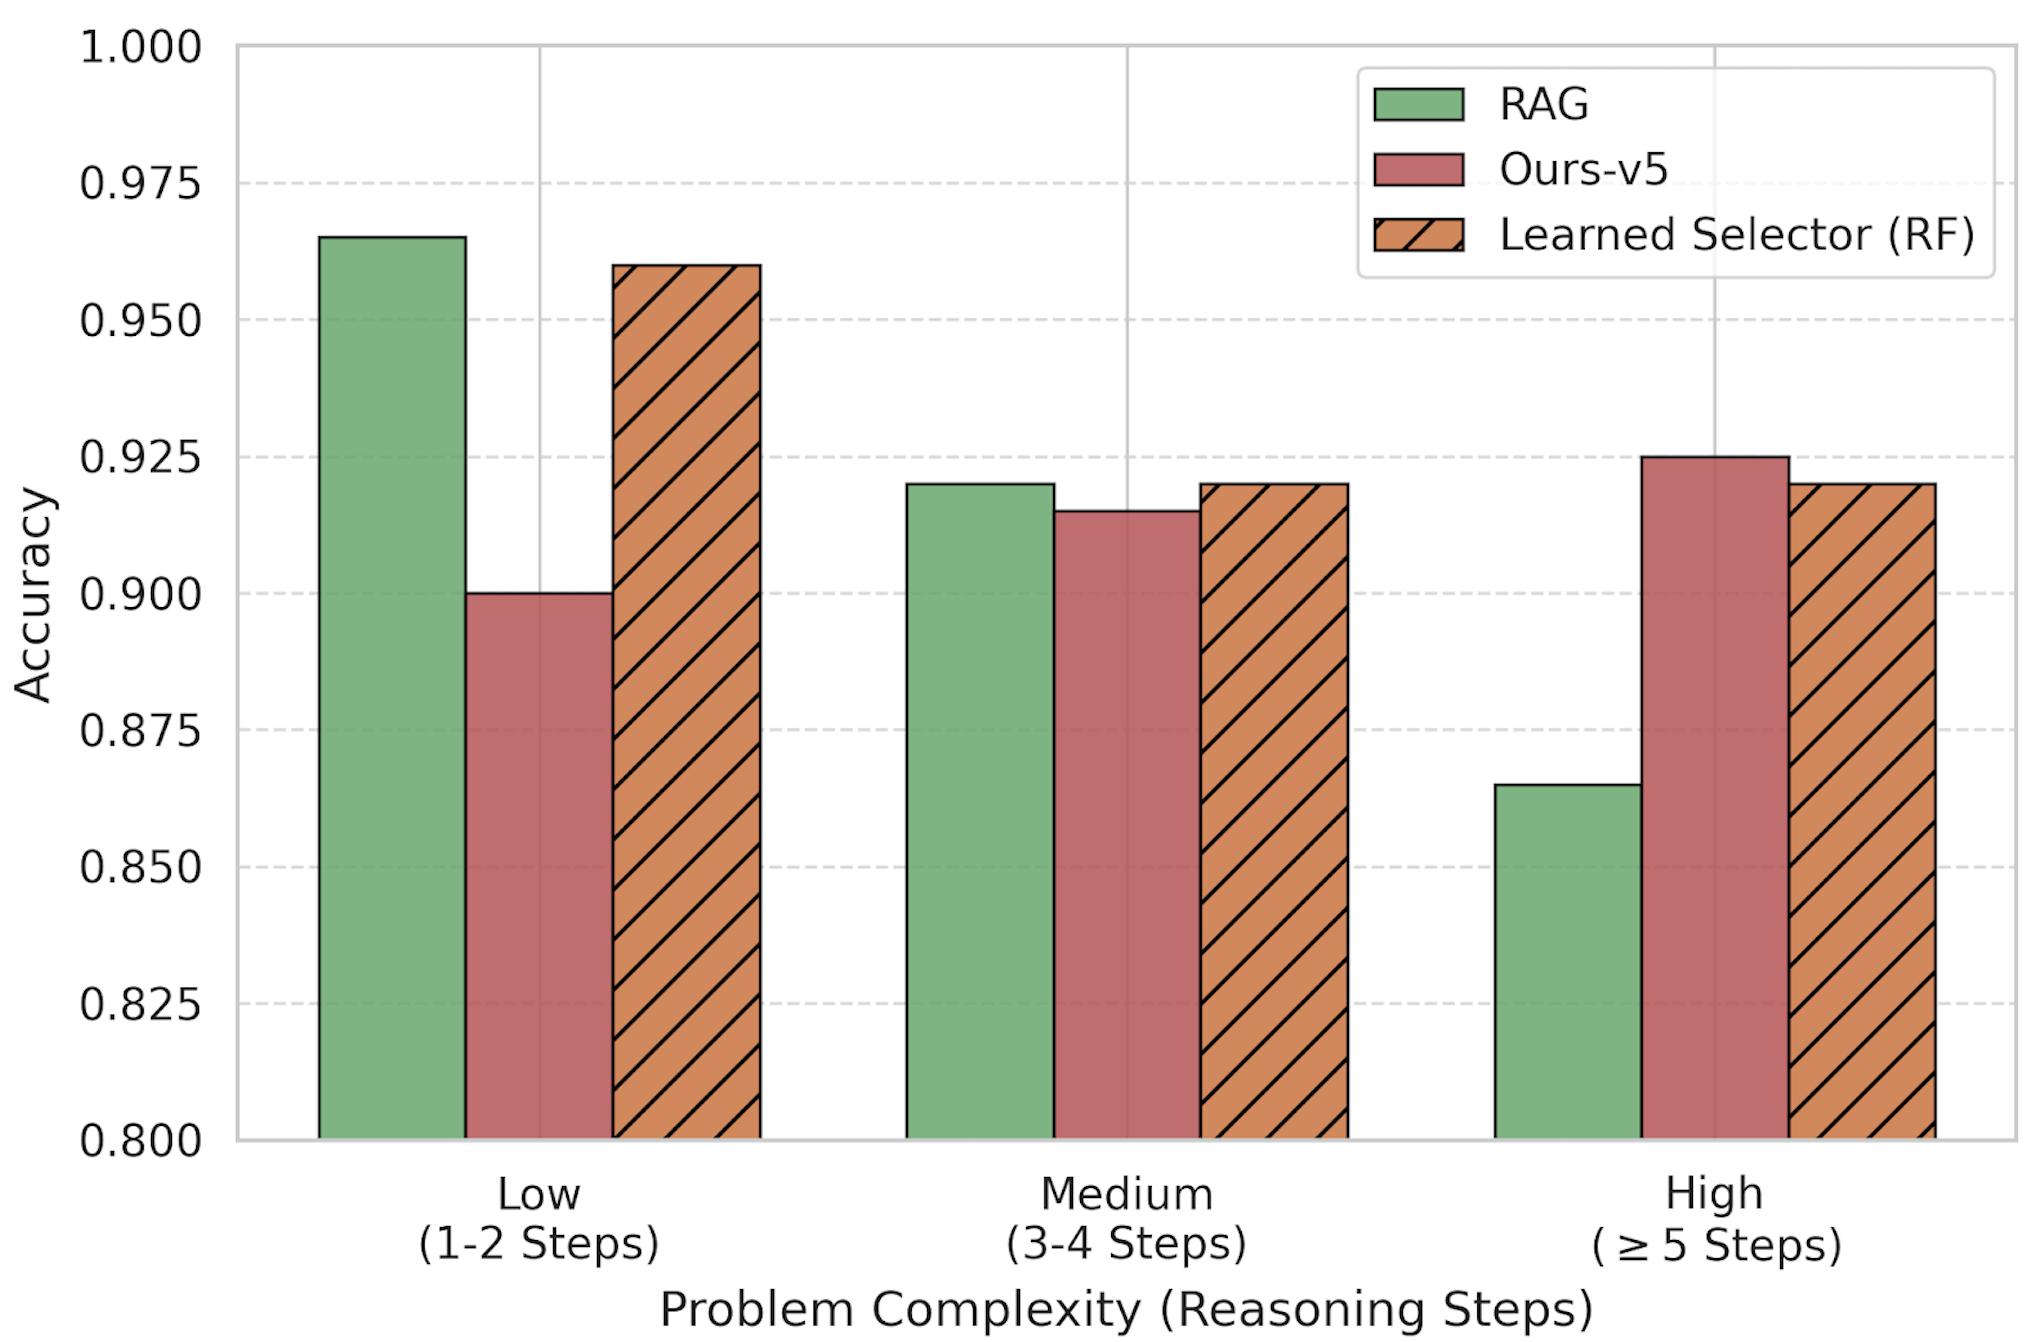
\includegraphics[width=0.72\linewidth]{figures/fig7_relative_line.png}
  \caption{Performance dynamics across different levels of problem complexity.}
  \label{fig:complexity_dynamics}
\end{figure}

Figure~\ref{fig:complexity_dynamics} shows that multi-agent debate better preserves performance on highly complex problems, while RAG is more robust on simpler ones, enabling the Learned Selector to dynamically route instances for improved overall performance.

\subsection{Case Study: Autonomous Error Correction}
To qualitatively demonstrate why routing complex queries to the multi-agent framework yields the gains reflected by the Oracle bound, we present a representative interaction transcript (see Box~\ref{box:revise_transcript}). In this GSM8K example, the Generator makes a common oversight (forgetting to multiply a daily rate by the number of days). The Critic intercepts the logical gap, and the Judge synthesizes the correct final output. This illustrates why debate-based revision is necessary beyond single-pass RAG on multi-step reasoning tasks.

\begin{center}
\fbox{%
\begin{minipage}{0.94\linewidth}
\small
\boxcaption{Transcript of the Multi-Agent Revise Phase}\label{box:revise_transcript}

\vspace{0.45em}
\textbf{Original Query.} John buys 3 apples a day. Each apple costs \$2. How much does he spend in a 5-day work week?

\vspace{0.45em}
\textbf{Generator's Initial Solution ($a_{\text{initial}}$).}
\begin{quote}
Step 1: John buys 3 apples a day, and each costs \$2.\\
Step 2: The daily cost is $3 \times 2 = 6$.\\
Step 3: Therefore, John spends \$6.\\
\textbf{Final Answer:} 6.
\end{quote}
\emph{Issue: The solution omits the 5-day temporal multiplier.}

\vspace{0.45em}
\textbf{Critic's Feedback ($c$).}
\begin{quote}
CRITICAL ERROR DETECTED. Your daily calculation is correct ($3 \times 2 = 6$). However, the prompt asks for total spending over a ``5-day work week.'' You stopped at daily cost and failed to multiply by 5.
\end{quote}

\vspace{0.45em}
\textbf{Judge's Final Solution ($a_{\text{final}}$).}
\begin{quote}
The Critic is correct: the initial solution misses the temporal multiplier.\\
\textbf{Corrected calculation:}\\
Daily cost $= 3 \times 2 = \$6$.\\
Total cost for 5 days $= \$6 \times 5 = \$30$.\\
\textbf{Final Answer:} 30.
\end{quote}
\end{minipage}%
}
\end{center}

\subsection{Error Analysis and Limitations}
While the adaptive framework improves reasoning reliability, the gap between the deployable Learned Selector (0.926) and the Oracle bound (0.950) reveals clear limitations. Through manual inspection of remaining errors, we identify two dominant failure sources:
\begin{itemize}
  \item \textbf{Negative transfer during retrieval.} Retrieved cases can be lexically similar but structurally mismatched, which may bias the Generator toward an incorrect formula template.
  \item \textbf{Echo chambers in multi-agent debate.} The Critic may occasionally miss subtle errors and output ``No Errors Found,'' leading the Judge to preserve a wrong draft; conversely, on hard items, the Critic can hallucinate non-existent errors and trigger harmful over-correction.
\end{itemize}
\begin{center}
  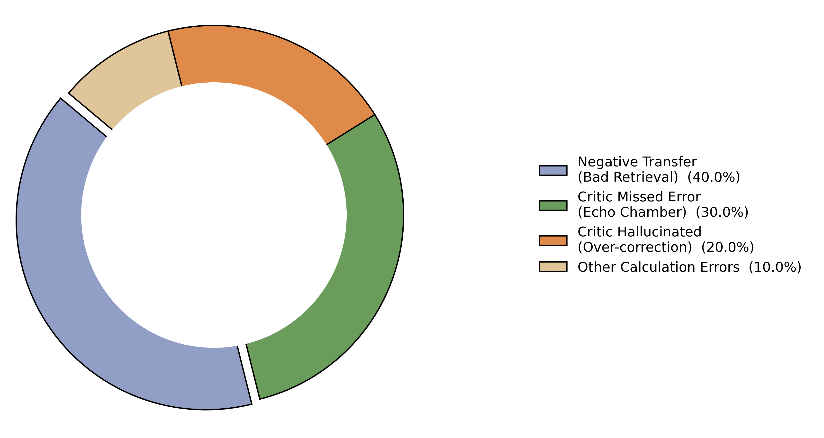
\includegraphics[width=0.78\linewidth]{figures/fig9_error_distribution.png}
  \captionof{figure}{Breakdown of failure modes in the remaining incorrect instances.}
  \label{fig:error_typology}
\end{center}

These observations suggest that developing richer confidence features for the Learned Selector and introducing more diverse, heterogeneous models for the Critic role are promising directions for future work.

\section{Conclusion and Future Work}
In this paper, we presented a framework that revitalizes classical Case-Based Reasoning (CBR) by integrating it with an LLM-driven multi-agent architecture. By explicitly mapping the 4R cycle (Retrieve, Reuse, Revise, Retain) into a dynamic reasoning workflow, the framework introduces a structured episodic-memory mechanism that most existing multi-agent systems do not explicitly maintain. A key contribution is the operationalization of the traditionally difficult Revise phase through autonomous interaction among Generator, Critic, and Judge agents.

Empirical results on GSM8K reveal a clear cost--performance trade-off. Blanket multi-agent debate is computationally expensive and can occasionally induce echo-chamber effects, while adaptive routing with a Learned Selector matches a strong RAG baseline (92.6\%) and reduces unnecessary token usage. The Oracle upper bound (95.0\%) further indicates substantial untapped gains from better routing between retrieval-only and debate-enhanced reasoning paths.

A key validity limitation is that current evidence is based on a 500-instance subset and a single backbone model (\texttt{gpt-4o-mini}); broader multi-model and full-test evaluations remain future work.

Future work will focus on narrowing the gap between the deployable Learned Selector and the Oracle bound through richer confidence features and uncertainty-aware signals. We also plan to move from a flat vector case base to a structured case graph that captures deeper relational and causal dependencies between reasoning steps. Finally, we will investigate heterogeneous agent collaboration (e.g., neural LLMs with symbolic solvers) to strengthen revise-stage reliability and reduce systematic blind spots.


\section*{Acknowledgments}
% Optional. Keep empty or add funding/collaboration credits.

\section*{Generative AI Statement}
The authors used generative AI tools to assist with language polishing, code prototyping, and figure scripting. All scientific claims, experimental design, implementation decisions, data analysis, and final manuscript content were reviewed and validated by the authors. The authors take full responsibility for the correctness and originality of this work.

\bibliographystyle{splncs04}
\bibliography{references}

\end{document}
